\documentclass[journal]{IEEEtran}
\usepackage{amsmath,amssymb}
\usepackage{booktabs}
\usepackage{cite}
\usepackage{graphicx}
\usepackage{tikz}
\usetikzlibrary{arrows.meta,positioning}
\usepackage{url}
\usepackage[hidelinks]{hyperref}
\usepackage{microtype}
% Generated by paper_evidence; source: ../evidence/summary.json
\newcommand{\StudyN}{266}
\newcommand{\Ours}{6220}
\newcommand{\Reference}{4066}
\newcommand{\Added}{2158}
\newcommand{\Lost}{4}
\newcommand{\Net}{2154}
\newcommand{\GainObservations}{141}
\newcommand{\AddedBytes}{402192}
\newcommand{\LostBytes}{1056}
\newcommand{\SignalN}{24}
\newcommand{\SignalOurs}{174}
\newcommand{\SignalReference}{111}
\newcommand{\SignalAdded}{63}
\newcommand{\SignalGainObservations}{6}
\newcommand{\NetPercent}{52.98}
\newcommand{\SignalPercent}{56.76}
\newcommand{\AudioHours}{34.11}

\newcommand{\code}[1]{\texttt{#1}}
\hypersetup{pdftitle={Telemetry Yield: A Resumable Receiver for Archived Satellite Audio},pdfauthor={Human authors to be supplied},pdfsubject={Unsubmitted research draft; historical CANVAS replay}}
\markboth{Telemetry Yield --- Research Draft, September 15, 2026}{Not submitted or peer reviewed}
\begin{document}
\title{Telemetry Yield: A Resumable Multi-Hypothesis Receiver for Recovering Telemetry from Archived Satellite Audio}
\author{Human authors and affiliations to be supplied\thanks{Unsubmitted research draft, version 2, September 15, 2026. This manuscript uses the IEEEtran journal layout; no IEEE acceptance, endorsement, assigned DOI or publication status is implied. Author contributions, affiliations, funding and conflicts require human review before submission.}}
\maketitle

\begin{abstract}
Archived radio observations allow additional receiver computation after a satellite pass has ended. We present Telemetry Yield, an offline Rust receiver combining complementary frontends, timing hypotheses, guarded channel estimation and sequence detection in a resumable task portfolio. A completed historical replay uses 266 CANVAS observations and supplies identical numerical audio to the native receivers, Dire Wolf and gr-satellites. The progressive receiver recovers 6220 AX.25 unnumbered-information packets, counted uniquely within observations, versus 4066 in the union of the two external receivers. It adds 2158 packets and misses four, a net increase of 52.98 percent; 141 observations have at least one addition. In a separately reported, metadata-defined signal-labelled subgroup, it recovers 174 packets versus 111, with 63 additions and no misses. These results incur substantially greater computation: mean concurrent-host process wall time is 192.39 seconds for the progressive receiver versus 3.69 and 3.94 seconds for the respective reference programs. A codec-conditioned experimental arm produces no incremental packets over its codec-disabled control. The previously exposed, single-mission cohort supports a retrospective systems result, not independent validation, equal-compute superiority, universal modulation coverage or a new optimal demodulation algorithm. A compact, checksum-bound companion bundle makes reported counts and subgroup arithmetic reproducible while explicitly separating them from full raw-artifact and runtime admission audits.
\end{abstract}
\begin{IEEEkeywords}
Satellite telemetry, software-defined radio, archived audio, sequence estimation, reproducible experiments, packet radio.
\end{IEEEkeywords}

\section{Introduction}
\IEEEPARstart{A}{ visible} satellite waveform need not produce a complete set of decoded packets. Timing error, receiver filtering, noise and channel distortion can cause different receiver configurations to recover different portions of a recording. Retaining the measurement creates an opportunity to revisit these decisions offline. The objective is additional validated received data, not fabricated payload completion or enhancement of information that the stored representation has irreversibly discarded.

This paper asks whether an explicit offline portfolio can add packets to controlled replays of established receivers and what the additional computation costs. A second question concerns the incremental value of residual prediction and codec-derived reliability. The questions require different comparisons: an overall portfolio comparison cannot establish the causal value of an individual branch.

The primary receiver, P, is the checkpointable progressive portfolio. I1 is a separate innovations receiver with codec conditioning disabled; I2 enables codec-derived and pooled calibration. Dire Wolf and gr-satellites provide external reference packet sets. SatNOGS supplies the original recordings, but the reference counts in this study are generated by our controlled replays, not taken from its production packet database.

The contributions are: an implemented finite portfolio with guarded, disjoint cross-packet channel transfer; an execution model that preserves completed work and result provenance under additional offline computation; and a completed, loss-aware historical evaluation with openly reported costs and a negative codec-ablation result. We do not claim invention of timing recovery, maximum-likelihood sequence estimation (MLSE), predictive whitening or weighted regression. Scientific priority for a narrowly defined algorithmic contribution is not established by this study.

\section{Context and Related Work}
MLSE for intersymbol-interference channels is established theory \cite{forney1972}. Gardner timing recovery is likewise a standard sampled-receiver technique \cite{gardner1986}. Estimation in autoregressive noise has longstanding treatment \cite{kay1994}. We use these families as building blocks. An exact trellis decision under a fitted effective channel is not evidence of a globally optimal receiver for the actual satellite waveform.

Dire Wolf is an AX.25 soundcard modem/TNC with packet-radio and APRS applications, including a GMSK/G3RUH path \cite{direwolf}. gr-satellites provides satellite-specific profiles and live or recorded input paths, including a distinction between real samples and complex IQ \cite{grsat}. SatNOGS is a broader ground-station network, client, scheduling and database stack \cite{satnogs}; a missing optional decoder profile is not proof that its native station receiver made no attempt. SatDump spans acquisition, satellite pipelines and downstream instrument/image products \cite{satdump}. These projects have different scopes, so a universal feature-ranking table would obscure the actual scientific comparison.

The WA8LMF test-medium description and Dire Wolf's associated results compilation are useful examples of published packet-radio comparison material \cite{wa8lmf,direwolfresults}. They are not a shared numerical scale with this CANVAS study. No Telemetry Yield score on that medium is reported. A comparison would need fixed track hashes, representation, modem settings and counting rules. Neither its packet totals nor an image from a different waveform can serve as a baseline for the experiment here.

\section{Receiver Design}
\subsection{Input and Output Contracts}
The evaluated receiver accepts mono post-frequency-demodulation audio for a configured 9600-baud FSK/GMSK link. IQ is a separate representation and entry point. A mono OGG recording cannot be treated as complex IQ to recover phase that was discarded before storage. Normal OGG preparation uses FFmpeg/ffprobe and a content-addressed float32 WAV; the historical comparison deliberately uses shared PCM16 instead, as described in Section~\ref{sec:evaluation}.

The receiver emits packet bytes, received integrity evidence, per-attempt provenance and completion state. It does not require a neural model. Mission-specific interpretation into physical measurements is downstream of framing and integrity; a plausible temperature or image is not a substitute for those checks.

\begin{figure}[t]
\centering
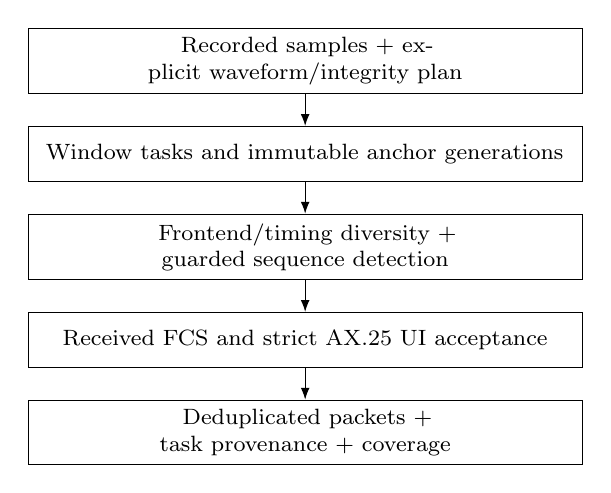
\begin{tikzpicture}[node distance=4mm, every node/.style={font=\footnotesize},box/.style={draw,align=center,text width=6.8cm,minimum height=7mm},arr/.style={-{Latex[length=1.5mm]}}]
\node[box] (in) {Recorded samples + explicit waveform/integrity plan};
\node[box,below=of in] (windows) {Window tasks and immutable anchor generations};
\node[box,below=of windows] (dsp) {Frontend/timing diversity + guarded sequence detection};
\node[box,below=of dsp] (valid) {Received FCS and strict AX.25 UI acceptance};
\node[box,below=of valid] (out) {Deduplicated packets + task provenance + coverage};
\draw[arr] (in)--(windows);\draw[arr] (windows)--(dsp);\draw[arr] (dsp)--(valid);\draw[arr] (valid)--(out);
\end{tikzpicture}
\caption{The evaluated progressive audio path. Durable task commits permit resumption. Generic IQ, FEC and companion image paths are separate capabilities, not additional evaluated arms hidden inside this diagram.}
\label{fig:architecture}
\end{figure}

\subsection{Frontend and Timing Diversity}
P processes six-second windows with a three-second hop. Overlap reduces boundary sensitivity; repeated detections are deduplicated when forming the observation-level packet set. Two frontends retain complementary responses: a legacy FIR/DC-removal path and a square-pulse path with DC rejection and RMS normalization.

Each frontend evaluates 160 fixed timing hypotheses: 32 phases at each of five clock offsets, $-500$, $-100$, 0, 100 and 500 ppm. Sixteen Gardner configurations combine two loop bandwidths, 0.02 and 0.06, with eight initial phases. The complete baseline therefore contains 352 attempts per window. A waveform-ranked quick prefix executes eight fixed timings and two Gardner configurations per frontend, or 20 attempts. The remaining baseline executes 332 attempts without repeating the prefix. Ranking uses signal samples rather than desired reference payloads.

\subsection{Guarded Channel Transfer}
Baseline packets require a valid received frame-check sequence (FCS) and strict AX.25 unnumbered-information (UI) structure. Their symbol decisions provide candidate training spans for an effective channel model. With binary symbols $x_n\in\{-1,+1\}$,
\begin{equation}
y_n=b+h_{-1}x_{n-1}+h_0x_n+h_{+1}x_{n+1}+e_n.
\label{eq:channel}
\end{equation}
Ridge-regularized fitting estimates the three taps and bias from at least 128 distinct guarded training symbols, subject to quality gates. This is a local post-FM audio approximation, not a complete physical GMSK channel model.

Source and target windows must use the same frontend, be disjoint with at least a one-second guard, and lie within 60 seconds. The nearest eligible source is chosen deterministically. Supplemental timing hypotheses combine transferred-clock phases and locally preferred candidates, deduplicating identical hypotheses. Archive packet bytes and external-decoder outputs are not supplied as training targets.

For gain $g\in\{0.75,1,1.5\}$, the white-residual sequence detector minimizes
\begin{equation}
\widehat{\boldsymbol{x}}_g=\arg\min_{\boldsymbol{x}}\sum_n
\left[y_n-g\left(b+\sum_{k=-1}^{1}h_kx_{n+k}\right)\right]^2.
\label{eq:mlse}
\end{equation}
A deterministic four-state Viterbi implementation uses full traceback and free initial/final states. This is sequence equalization, not convolutional FEC decoding. Model mismatch remains even when the configured metric is optimized exactly.

\subsection{Supplemental Branches and Evidence Separation}
A bounded blind branch alternates sequence decisions and channel fitting from multiple initial seeds. Separate waveform-fit checks reject poor models. A multi-anchor branch combines compatible local estimates using quality and time-distance weights. Neither a low fitting error nor a blind channel estimate counts as a validated packet.

The baseline, nearest-anchor, blind and multi-anchor outputs form an additive union. Early supplemental stages use an immutable quick-prefix anchor generation; final stages use the completed baseline generation. Supplemental packets do not recursively create new training anchors. Preserving the native baseline does not imply preservation of every packet found by an external receiver. No CRC-guided bit repair is used in the evaluated progressive path.

Temporal separation prevents direct fitting to the target packet but does not make adjacent windows independent. Source frontend/timing choices still depend on their source windows. These qualifications matter both for model validation and for claims of statistical novelty.

\subsection{Resumable Execution}
Quick, deep and full modes allocate time to the same finite task bank. Default quick/deep invocation budgets are 3000/60000 ms. Preparation, hashing and checkpoint verification consume the budget. Scheduling and cleanup can exceed it; these are supervised budgets, not hard real-time latency guarantees.

Manifests bind input, prepared samples, executable and policy identities. Complete tasks are durably committed, while partial task execution may be retried after interruption. Compatible later invocations continue from committed work. Atomic snapshots expose the current packet union and coverage; an incomplete run is different from a complete zero-packet observation. Bounded caches reuse numerical frontend/timing representations without pruning the configured bank.

\section{Separate Codec Experiment}
I1/I2 retain an adaptive baseline and additional matched-white/residual-predictive lanes. Their portfolio is not P's complete progressive blind/multi-anchor bank. I2 additionally evaluates codec-conditioned and pooled-codec reliability models.

For residuals in \eqref{eq:channel}, the candidate innovations objective has the form
\begin{equation}
J(\boldsymbol{x})=\sum_n\frac{\left(e_n-\sum_{j=1}^{p}a_je_{n-j}\right)^2}{v_n},
\quad v_n>0,
\label{eq:innovations}
\end{equation}
with bounded orders $p\in\{0,1,2\}$, source-based fitting and disjoint validation. The constant-weight, order-zero case delegates to the original detector to preserve arithmetic. Prediction and reliability weighting are established techniques, not by themselves a new algorithm.

Codec conditioning uses original Vorbis packet/frame information as proxies for local reliability, including encoded bits per decoded sample and changes in decoded-frame lengths. These are not known quantization errors or a complete codec-state reconstruction. Alignment is checked against the decoded sample coordinates. Pooling requires multiple disjoint source windows and independently received anchors; rejected calibration disables the optional branch rather than invalidating an observation. Because I2 sees original-container side information, its information access differs from the other arms even though their numerical PCM inputs match.

\section{Historical Evaluation}\label{sec:evaluation}
\subsection{Cohort and Exposure}
All \StudyN{} observations completed the five-arm replay. They span 15 UTC dates, 161 station identifiers and \AudioHours{} hours of audio. The cohort was amended from 500 selected CANVAS observations by excluding 234 under recorded prior-exposure/proximity rules, including a 120-minute same-satellite guard. It is not representative of all missions, modulation families or observation outcomes.

The optimized executable campaign is a disclosed repeat after a performance-only restart. Earlier partial results had been inspected. Finishing the trial does not restore unseen-holdout status. The evidence bundle includes the receiver freeze, historical protocol and prior-evaluation exposure record. A complete local reporting export was prepared on September 15, 2026; no new decoder execution was performed to prepare this paper revision.

\subsection{Shared Input and Comparator Settings}
Each original OGG is converted once into a shared signed PCM16 WAV, retaining sample rate/channels without resampling, per-arm gain adjustment or hand-selected cropping. Bitexact container flags provide a WAV compatible with the installed reference program. Conversion belongs to the input-preparation protocol, not an advantage applied to only one waveform arm.

Dire Wolf runs \code{atest -B 9600 -F 0 -h}, disabling bit repair. gr-satellites uses the frozen generic FSK 9600 / AX.25 G3RUH profile with network submission disabled. Its result is not a maximum over every available mission profile and tuning option. Binary identities, profile content and selected runtime dependencies are frozen; this is not a complete hermetic operating-system image.

The campaign uses four observation workers, two threads per native arm and a 900-second outer arm cap. P has an 880000-ms internal budget and must complete its required bank. Arm order rotates. Successful final process wall times include startup but exclude common conversion; they were measured on a shared host. Different parallelism, retries and contention prevent interpreting aggregate wall sums as campaign duration or isolated CPU efficiency.

\subsection{Packet Identity and Metrics}
Let $P_i,D_i,G_i$ be exact FCS-stripped UI PDU byte sets for observation $i$, and $B_i=D_i\cup G_i$. Repetition within an observation counts once; the same bytes in a different observation count again. Define
\begin{align}
A&=\sum_i|P_i\setminus B_i|, & L&=\sum_i|B_i\setminus P_i|,\\
\Delta&=A-L, & R&=100\,\frac{\Delta}{\sum_i|B_i|}.
\label{eq:metrics}
\end{align}
$R$ is undefined for an empty reference denominator. Additions, losses and the number of observations affected are reported separately. PDU byte totals include headers but exclude FCS; they are not application-only scientific measurements or a count of globally new telemetry.

Native received FCS is retained and independently recomputed by the artifact analyzer. External PDUs omit it and rely on the external decoder's internal FCS check, followed by structural and exact-byte comparison. This asymmetry is explicit. CRC is not transmitter authentication, and a large correlated hypothesis bank does not justify a naive independent-trial false-acceptance calculation.

\subsection{Signal Subgroup and Dependence}
The separately tracked subgroup is frozen metadata with \code{waterfall\_status=with-signal}, not a condition on native packet recovery. There are 24 such labels, three without-signal labels and 239 unknowns. Unknown does not mean no transmission. This subgroup was requested after initial results and is exploratory; labels are not independent signal truth or spacecraft attribution.

Stations, overlapping passes, dates and repeated payloads induce dependence. The archived analyzer supplies descriptive paired component-bootstrap sensitivity intervals with 10000 draws at grouping gaps of 0, 1800 and 7200 seconds. It explicitly leaves independence uncertified. These intervals are not used as a significance gate or evidence for generalization to all SatNOGS recordings.

\section{Results}
\subsection{Packet Yield and Cost}
\begin{table}[t]
\caption{Complete historical replay: observation-level unique PDUs and final process wall sums. Concurrent-host timings exclude shared conversion; they are not campaign elapsed time.}
\label{tab:yield}
\centering\footnotesize
% Generated from the frozen evidence; final process wall sums, not elapsed campaign time.
\begin{tabular}{lrrr}
\toprule Arm & PDUs & Wall sum (s) & Mean (s)\\
\midrule
Dire Wolf & 4029 & 982.38 & 3.69\\
gr-satellites & 2514 & 1047.27 & 3.94\\
Progressive P & 6220 & 51175.17 & 192.39\\
Innovations I1 & 6420 & 38350.82 & 144.18\\
Innovations I2 & 6420 & 39130.71 & 147.11\\
\bottomrule
\end{tabular}

\end{table}

P recovers \Ours{} packets versus \Reference{} in $B$, with \Added{} additions and \Lost{} losses: \Net{} net additional packets or \NetPercent\%. At least one addition occurs in \GainObservations{}/\StudyN{} observations (53.01\%). Four observations contain losses; three of these also contain additions. Thus larger totals do not imply a superset of reference packets. Table~\ref{tab:yield} reports all five arms rather than selecting only favorable comparisons.

The added PDU bytes total \AddedBytes{}, while missed PDU bytes total \LostBytes{}. The sum over the complete progressive set is 1159176 PDU bytes excluding FCS. These are received protocol-byte quantities, not necessarily distinct physical measurements. Without transmitted ground truth, neither packet recall nor the fraction of all available telemetry is known.

\begin{figure}[t]
\centering
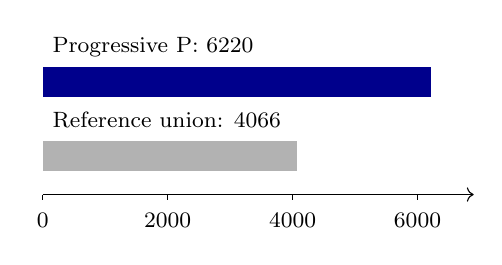
\begin{tikzpicture}[x=0.0008cm,y=0.85cm,every node/.style={font=\footnotesize}]
\fill[black!30] (0,0) rectangle (\Reference,0.45);
\fill[blue!55!black] (0,1.1) rectangle (\Ours,1.55);
\node[anchor=west] at (0,1.86) {Progressive P: \Ours{}};
\node[anchor=west] at (0,0.76) {Reference union: \Reference{}};
\draw[->] (0,-0.35)--(6900,-0.35);
\foreach \x in {0,2000,4000,6000}{\draw (\x,-0.35)--(\x,-0.43);\node[anchor=north] at (\x,-0.48){\x};}
\end{tikzpicture}
\caption{Historical packet counts on a common zero-origin scale. P adds \Added{} packets but misses \Lost{}; its larger bar is not a superset guarantee or an equal-compute comparison. The cohort was previously exposed.}
\label{fig:yield}
\end{figure}

P averages 192.39 seconds per recording versus 3.69 seconds for Dire Wolf and 3.94 for gr-satellites. Its summed wall time is approximately 52 times Dire Wolf's and 49 times gr-satellites'. The extra recovery has a substantial cost. Being shorter than the recorded audio in aggregate does not establish streaming latency, hard-deadline compliance or an isolated acceleration factor.

At the 7200-second dependence grouping, the descriptive net-percentage bootstrap interval is 43.14--63.39\%, using 44 components. The estimate is conditional on the selected, historically exposed sample. Its positive endpoints do not resolve selection bias or certify independence.

\subsection{Signal-Labelled Observations}
All \SignalN{} signal-labelled observations are complete. P yields \SignalOurs{} packets versus \SignalReference{} in $B$: \SignalAdded{} additions, zero losses, and \SignalPercent\% net increase. \SignalGainObservations{} of the 24 observations have additions. This result is rederived from the full committed cohort, not an earlier partial progress report. The small, post-hoc subgroup is reported alongside the main result rather than promoted as a separate confirmatory study.

\subsection{Negative Codec-Ablation Result}
I1 and I2 each yield 6420 packets and have identical observation-level sets throughout the cohort: zero additions and zero losses attributable to enabling I2. The data therefore provide no incremental packet-yield evidence for codec conditioning/pooling in this comparison.

I2 adds 2359 packets and misses five relative to $B$, a net 2354 or 57.89\%. This is a result for its whole portfolio, not for its codec branch. Because I1/I2 and P use different portfolios, the 200-packet aggregate difference cannot isolate a specific improvement. Post-hoc unioning of their outputs would also be exploratory and would require a newly frozen operating policy for independent evaluation.

\subsection{Missed Reference Packets}
The four P losses occur in observations 14785751, 14798555, 14834989 and 14848596, one PDU each. Their addition/loss counts are respectively 19/1, 19/1, 0/1 and 15/1. Listing these cases prevents an aggregate gain from concealing a complete local regression, such as the zero-versus-one result in 14834989. The summary does not identify the physical cause of each missed packet; waveform-level trace-back remains required.

\section{Reproducibility and Engineering Status}
The current repository separates the receiver library, CLI schema/dispatch, DSP, protocol/FEC layers, compute backend and artifact auditing. Generic IQ paths implement BPSK, QPSK and OQPSK with explicit plans; selected CSP, CCSDS TM/AOS/USLP, Reed--Solomon and LDPC functionality exists. These are not the paths evaluated in Table~\ref{tab:yield}. No broad orbital PSK gain or complete mission-service coverage follows from the audio result.

CPU is the default. Optional CUDA acceleration currently covers real/complex FIR filtering, including PSK matched filtering, while FFT, synchronization, sequence detection and FEC remain on CPU. GPU requests fail explicitly when unavailable. Host-side tests and NVRTC compilation are not hardware execution. Actual device parity, error handling and end-to-end speedup are still open qualification gates.

A separate September 14 refactor qualification preserved 20 complete frames and 1372 scientific task results on one known development recording across the compared CPU builds/settings. It also passed 195 bit-exact FIR qualification cases. These are engineering regression checks, not a rerun of this historical cohort on the current executable, a GPU result or an independent research replication.

The companion reporting tool recomputes exact-set additions/losses from committed per-observation PDU sets, checks them against the final yield analyzer, and checks time sums against the cost report. It exports counts, source/result hashes, source URLs, a profile and frozen receiver identities. The portable verifier checks these bundle hashes and count arithmetic without access to the large laboratory archive.

This distinction limits the evidence claim. The compact bundle does not contain all raw waveforms, original FCS, task artifacts or external logs. Its successful verification is not a fresh waveform decode. The final yield analyzer rederives native CRC and external hex/KISS sets but relies on separate runner/control audits for full task policy and runtime admission. Its \code{publication\_ready} and independence-certification flags remain false. Hash consistency is not authentication against wholesale replacement of the evidence tree.

\section{Limitations and Next Evaluation}
The study is retrospective, single-mission and previously exposed. It does not support a population-wide recovery percentage, a sensitivity improvement in dB, superiority at equal compute or an assertion that every supported protocol is field-qualified. More search can increase yield while also increasing cost and the opportunity for false acceptance.

A stronger scientific evaluation should freeze code, cohort, acceptance policy and comparison budgets before inspecting outcomes. Unexposed historical recordings can provide this separation; waiting for future observations is unnecessary. Selection should retain zero-yield and difficult observations, report missingness, and group related passes/stations to limit leakage. No tuning should use held-out payloads or successful packet counts.

Matched ablations must hold input precision, frontends, timing banks, acceptance rules and resources fixed while removing one component. Full-policy no-transmission, wrong-profile and controlled-corruption tests should quantify false acceptance. Representative added and missed packets need independent waveform trace-back and mission interpretation. Unchanged or negative results, including the codec finding here, should remain in the record.

For deployment, the remaining work includes clean-source installation, controlled releases, long-duration recovery/failure exercises, environment pinning and accountable maintenance. For efficiency, isolated repeated paired timing should include CPU usage, GPU identity, startup/transfers, tail latency and identical packet/task outputs. A polished repository and successful local tests do not by themselves establish enterprise service qualification.

\section{Conclusion}
An explicit offline receiver portfolio recovers additional packets from the same numerical satellite audio used by two configured reference receivers. Across the completed 266-observation historical cohort, P provides a 52.98\% net packet increase with four reference packets missed and substantially greater computation. The separately reported signal-labelled subgroup also shows additions, while the codec-enabled experiment yields no incremental packets over its control. These findings motivate a complementary, auditable second-pass workflow and a stronger independent evaluation, not a claim of universal replacement or revolutionary new demodulation theory.

\section*{Data and Software Availability}
The repository includes this manuscript, BibTeX references, generated result tables, a compact evidence bundle and its Rust reporting tool. Original OGG locators and hashes are supplied per observation; availability of remote originals is not guaranteed. No public Git remote, archival DOI, independently reproduced release or completed distribution clearance is claimed. The full laboratory artifacts and frozen runtime closure must be made available under author-approved arrangements for a complete reproduction. Version 1 remains an archived interim snapshot; this version reports the complete cohort.

\section*{Acknowledgment and Draft Disclosure}
We acknowledge the SatNOGS station operators and the contributors to Dire Wolf, gr-satellites and other referenced software. No endorsement is implied. OpenAI ChatGPT/Codex assisted throughout this draft with prose, organization, method descriptions, equations, figures, tables, bibliography and reporting code; receiver and benchmark implementation also included such assistance. Figures/tables derive from the recorded experiment or depict the implemented architecture, not invented observations. Human authors must review the complete technical content and attribution before submission. This disclosure follows IEEE guidance on generated content \cite{ieeeguidance}; AI systems are not authors. Authorship, affiliations, funding and competing-interest statements remain to be supplied.

\bibliographystyle{IEEEtran}
\bibliography{references}
\end{document}
